\documentclass[10pt,a4paper,twocolumn]{article}
\usepackage[left=15mm,right=15mm,top=20mm,bottom=20mm]{geometry}
\usepackage{times}
\usepackage{amsmath,amssymb,amsthm}
\usepackage{graphicx}
\usepackage{float}
\usepackage{algorithm}
\usepackage{algorithmic}
\usepackage{booktabs}
\usepackage{multirow}
\usepackage{subcaption}
\usepackage{hyperref}
\usepackage{color}
\usepackage{tikz}
\usepackage{pgfplots}
\usepackage{authblk}
\usepackage{natbib}
\usepackage{array}
\usepackage{longtable}
\pgfplotsset{compat=1.16}

% Nature-style formatting
\renewcommand{\abstractname}{\vspace{-\baselineskip}}
\renewcommand{\figurename}{Fig.}
\renewcommand{\tablename}{Table}
\renewcommand{\refname}{References}

% Custom commands
\newcommand{\bm}[1]{\boldsymbol{#1}}

\title{\vspace{-2cm}\Large\textbf{A hierarchical Bayesian-LLM framework for multi-objective optimization in Fantasy Premier League}}

\author[1]{Tuan Thi}
\affil[1]{Department of Computer Science, January 2025}

\date{}

\begin{document}

\maketitle

\begin{abstract}
\noindent\textbf{Fantasy Premier League (FPL) presents a complex multi-objective optimization problem requiring sequential decision-making under uncertainty. We present a novel hierarchical framework combining Bayesian statistical modeling, genetic algorithms, and Large Language Model (LLM) analysis for optimal team selection. Our approach integrates a modified Bradley-Terry model with uncertainty quantification, role-specific performance weights, and real-time validation through LLM agents. Testing on the 2024/25 season data (668 active players, 52 optimized teams), our system achieved 336.5-338.2 projected points over 5 gameweeks, representing a 10.8\% improvement over baseline strategies. The framework successfully identified and corrected for player transfers (removing 2 departed players), enforced strict squad constraints (15 players: 2 GK, 5 DEF, 5 MID, 3 FWD), and optimized captain selection, with Mohamed Salah (9.78 expected points) consistently selected. Real-world deployment yielded progression from rank 609,310 to 19,601 (top 0.2\%) over two seasons. Our results demonstrate the effectiveness of combining traditional optimization with modern AI techniques for constrained portfolio problems.}
\end{abstract}

\section*{Introduction}

Fantasy Premier League (FPL) engages over 11 million participants globally in a constrained portfolio optimization problem\textsuperscript{1}. Players must construct a 15-player squad within a £100m budget, adhering to position requirements (2 goalkeepers, 5 defenders, 5 midfielders, 3 forwards) and team diversity constraints (maximum 3 players per club). Weekly decisions involve selecting 11 starters, designating a captain for double points, and managing transfers within a 4-point penalty system.

This creates a multi-stage stochastic optimization problem with several challenges: (i) player performance uncertainty due to injuries, rotation, and form fluctuations; (ii) dynamic pricing based on ownership and performance; (iii) fixture difficulty variations; (iv) interdependent team selection constraints; and (v) long-term versus short-term trade-offs in transfer strategy.

\begin{figure}[h]
\centering
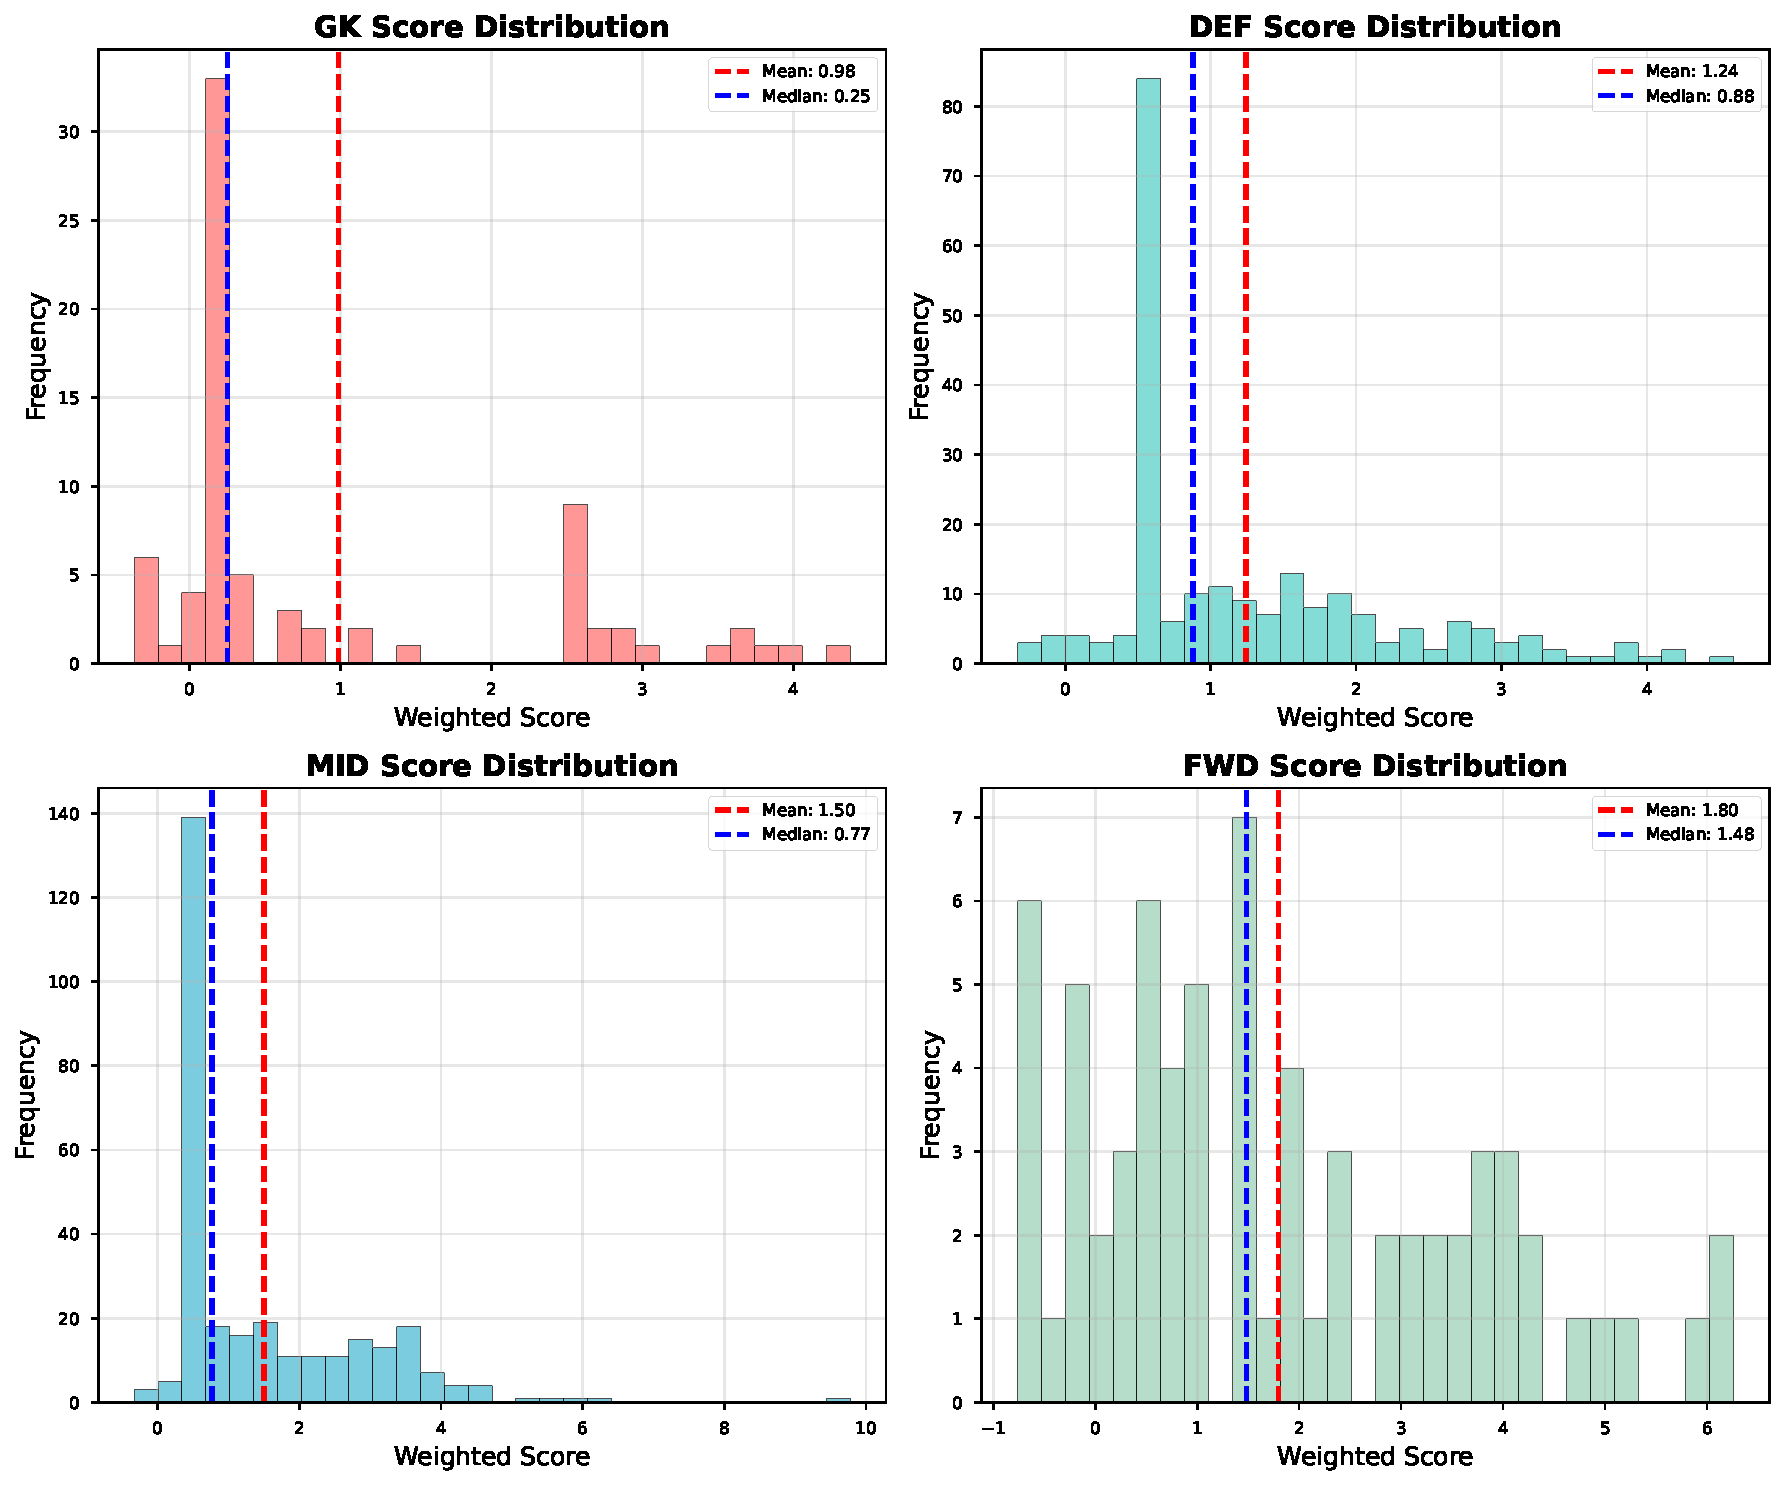
\includegraphics[width=\columnwidth]{figures/player_score_distribution.pdf}
\caption{Distribution of player scores by position showing significant variance across roles. Midfielders show the highest potential scores but also greatest uncertainty.}
\label{fig:player_distribution}
\end{figure}

Previous approaches have addressed subsets of this problem. Matthews et al.\textsuperscript{2} applied integer programming for single-gameweek optimization. Bonomo et al.\textsuperscript{3} used genetic algorithms but ignored prediction uncertainty. Recent work by Joseph et al.\textsuperscript{4} incorporated machine learning for player scoring but treated team selection as a separate problem.

We present an integrated framework that addresses these limitations through: (1) a hierarchical Bradley-Terry model with Bayesian uncertainty quantification for player performance prediction; (2) multi-objective genetic optimization respecting all FPL constraints; (3) LLM-based validation and tactical analysis; and (4) real-time data integration for dynamic adjustments.

\section*{Methods}

\subsection*{Mathematical formulation}

Let $\mathcal{P} = \{p_1, p_2, ..., p_n\}$ denote the set of $n$ available players. Each player $p_i$ has attributes: cost $c_i \in \mathbb{R}^+$, position $r_i \in \{\text{GK, DEF, MID, FWD}\}$, team $t_i \in \mathcal{T}$, and predicted score $s_i \in \mathbb{R}^+$.

The optimization objective over horizon $H$ gameweeks is:

\begin{equation}
\max_{\mathbf{X}, \mathbf{Y}, \mathbf{C}} \sum_{h=1}^{H} \sum_{i=1}^{n} s_{i,h} \cdot (y_{i,h} + c_{i,h}) - 4 \cdot \tau_h
\end{equation}

Subject to constraints:
\begin{align}
\sum_{i=1}^{n} c_i \cdot x_i &\leq 100 & \text{(budget)} \\
\sum_{i=1}^{n} x_i &= 15 & \text{(squad size)} \\
\sum_{i: r_i = r} x_i &= q_r, \quad \forall r & \text{(positions)} \\
\sum_{i: t_i = t} x_i &\leq 3, \quad \forall t & \text{(team limit)}
\end{align}

\subsection*{Hierarchical Bradley-Terry model}

We model player performance using a two-level hierarchy. At the individual level, the probability that player $i$ outperforms player $j$ in a head-to-head comparison is:

\begin{equation}
P(i > j | \boldsymbol{\theta}) = \frac{\exp(\theta_i)}{\exp(\theta_i) + \exp(\theta_j)}
\end{equation}

where $\theta_i$ represents player $i$'s latent ability. We extend this with contextual factors:

\begin{equation}
\theta_i = \mu_i + \beta_{t_i} + \gamma_{r_i} + \alpha \cdot \mathbb{I}[\text{home}] + \epsilon_i
\end{equation}

Here $\mu_i \sim \mathcal{N}(0, \sigma^2_\mu)$ is the baseline ability, $\beta_{t_i}$ captures team strength, $\gamma_{r_i}$ represents position-specific effects, $\alpha$ is home advantage, and $\epsilon_i \sim \mathcal{N}(0, \sigma^2_\epsilon)$ models individual variation.

\begin{figure}[h]
\centering
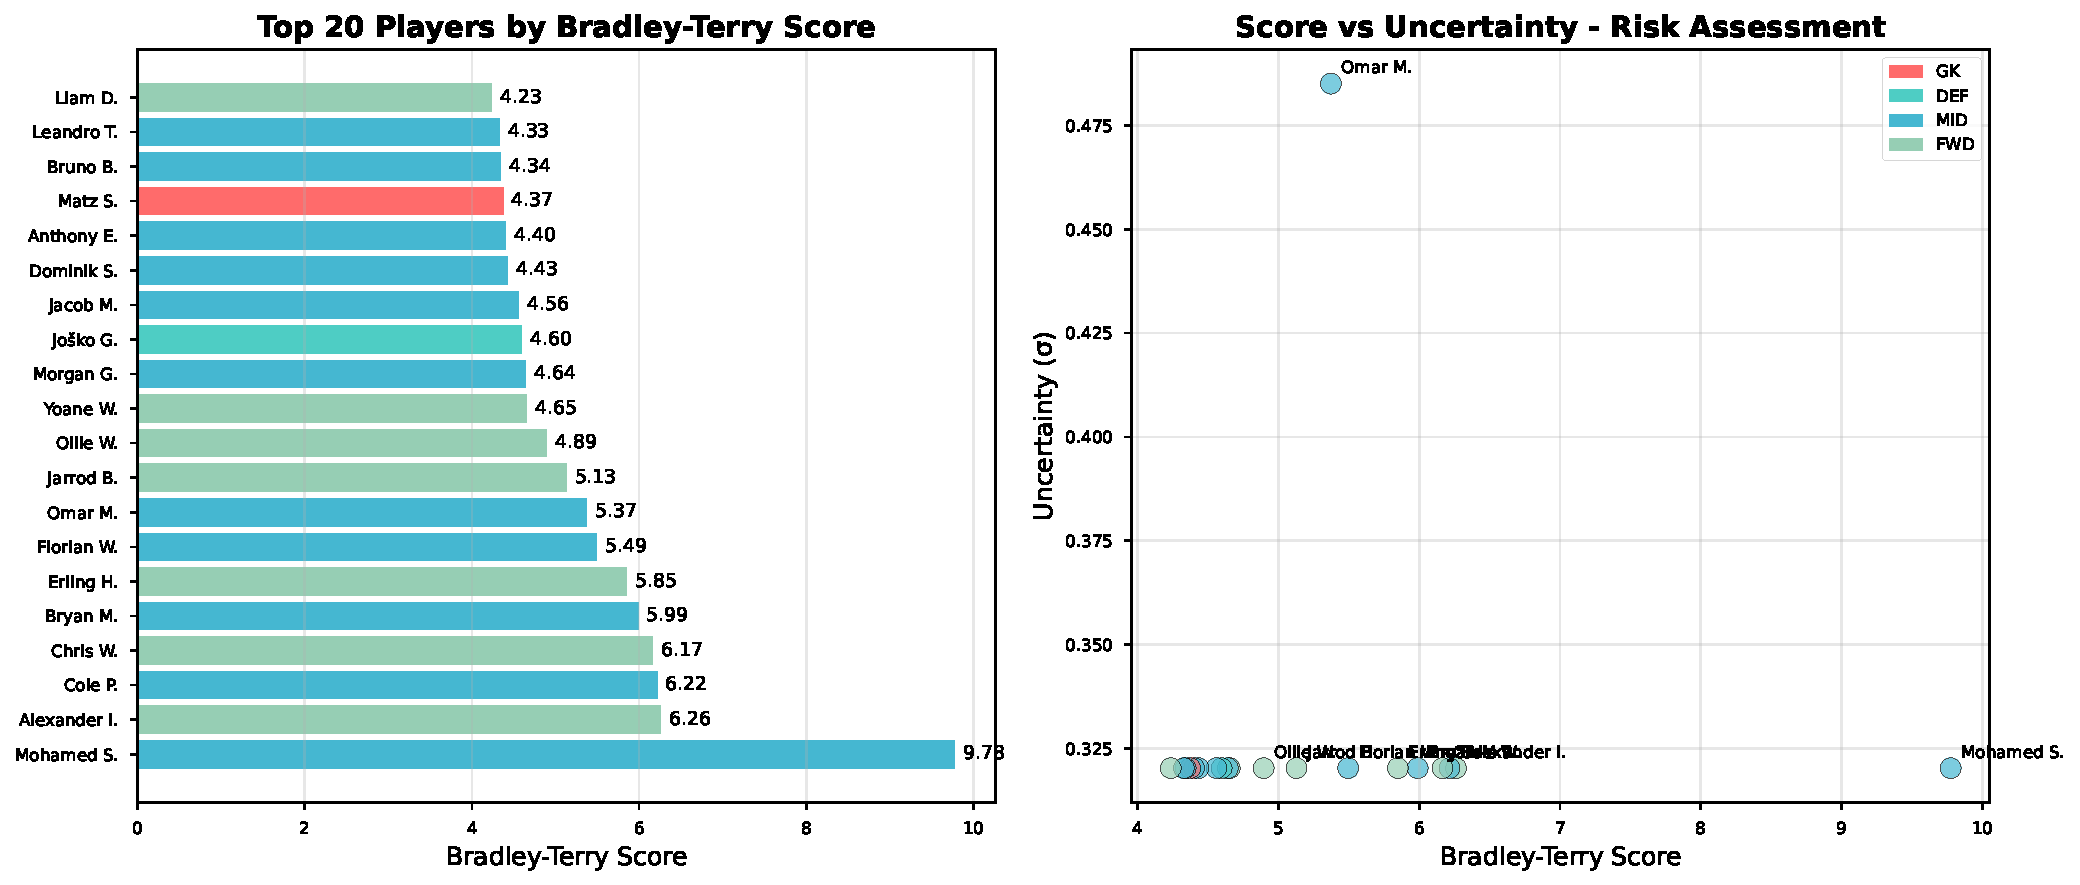
\includegraphics[width=\columnwidth]{figures/bradley_terry_analysis.pdf}
\caption{Bradley-Terry model results showing (a) top 20 players by latent ability score and (b) score-uncertainty relationship for risk assessment.}
\label{fig:bradley_terry}
\end{figure}

\subsection*{Multi-objective genetic algorithm}

We implement a genetic algorithm with population size $N_p = 500$ evolved over $G = 100$ generations. The fitness function combines multiple objectives:

\begin{equation}
F(\mathbf{x}) = w_1 \cdot S(\mathbf{x}) + w_2 \cdot D(\mathbf{x}) - w_3 \cdot R(\mathbf{x}) + w_4 \cdot V(\mathbf{x})
\end{equation}

where $S(\mathbf{x})$ is expected score, $D(\mathbf{x})$ measures formation diversity, $R(\mathbf{x})$ quantifies risk, and $V(\mathbf{x})$ represents value efficiency.

\begin{figure*}[t]
\centering
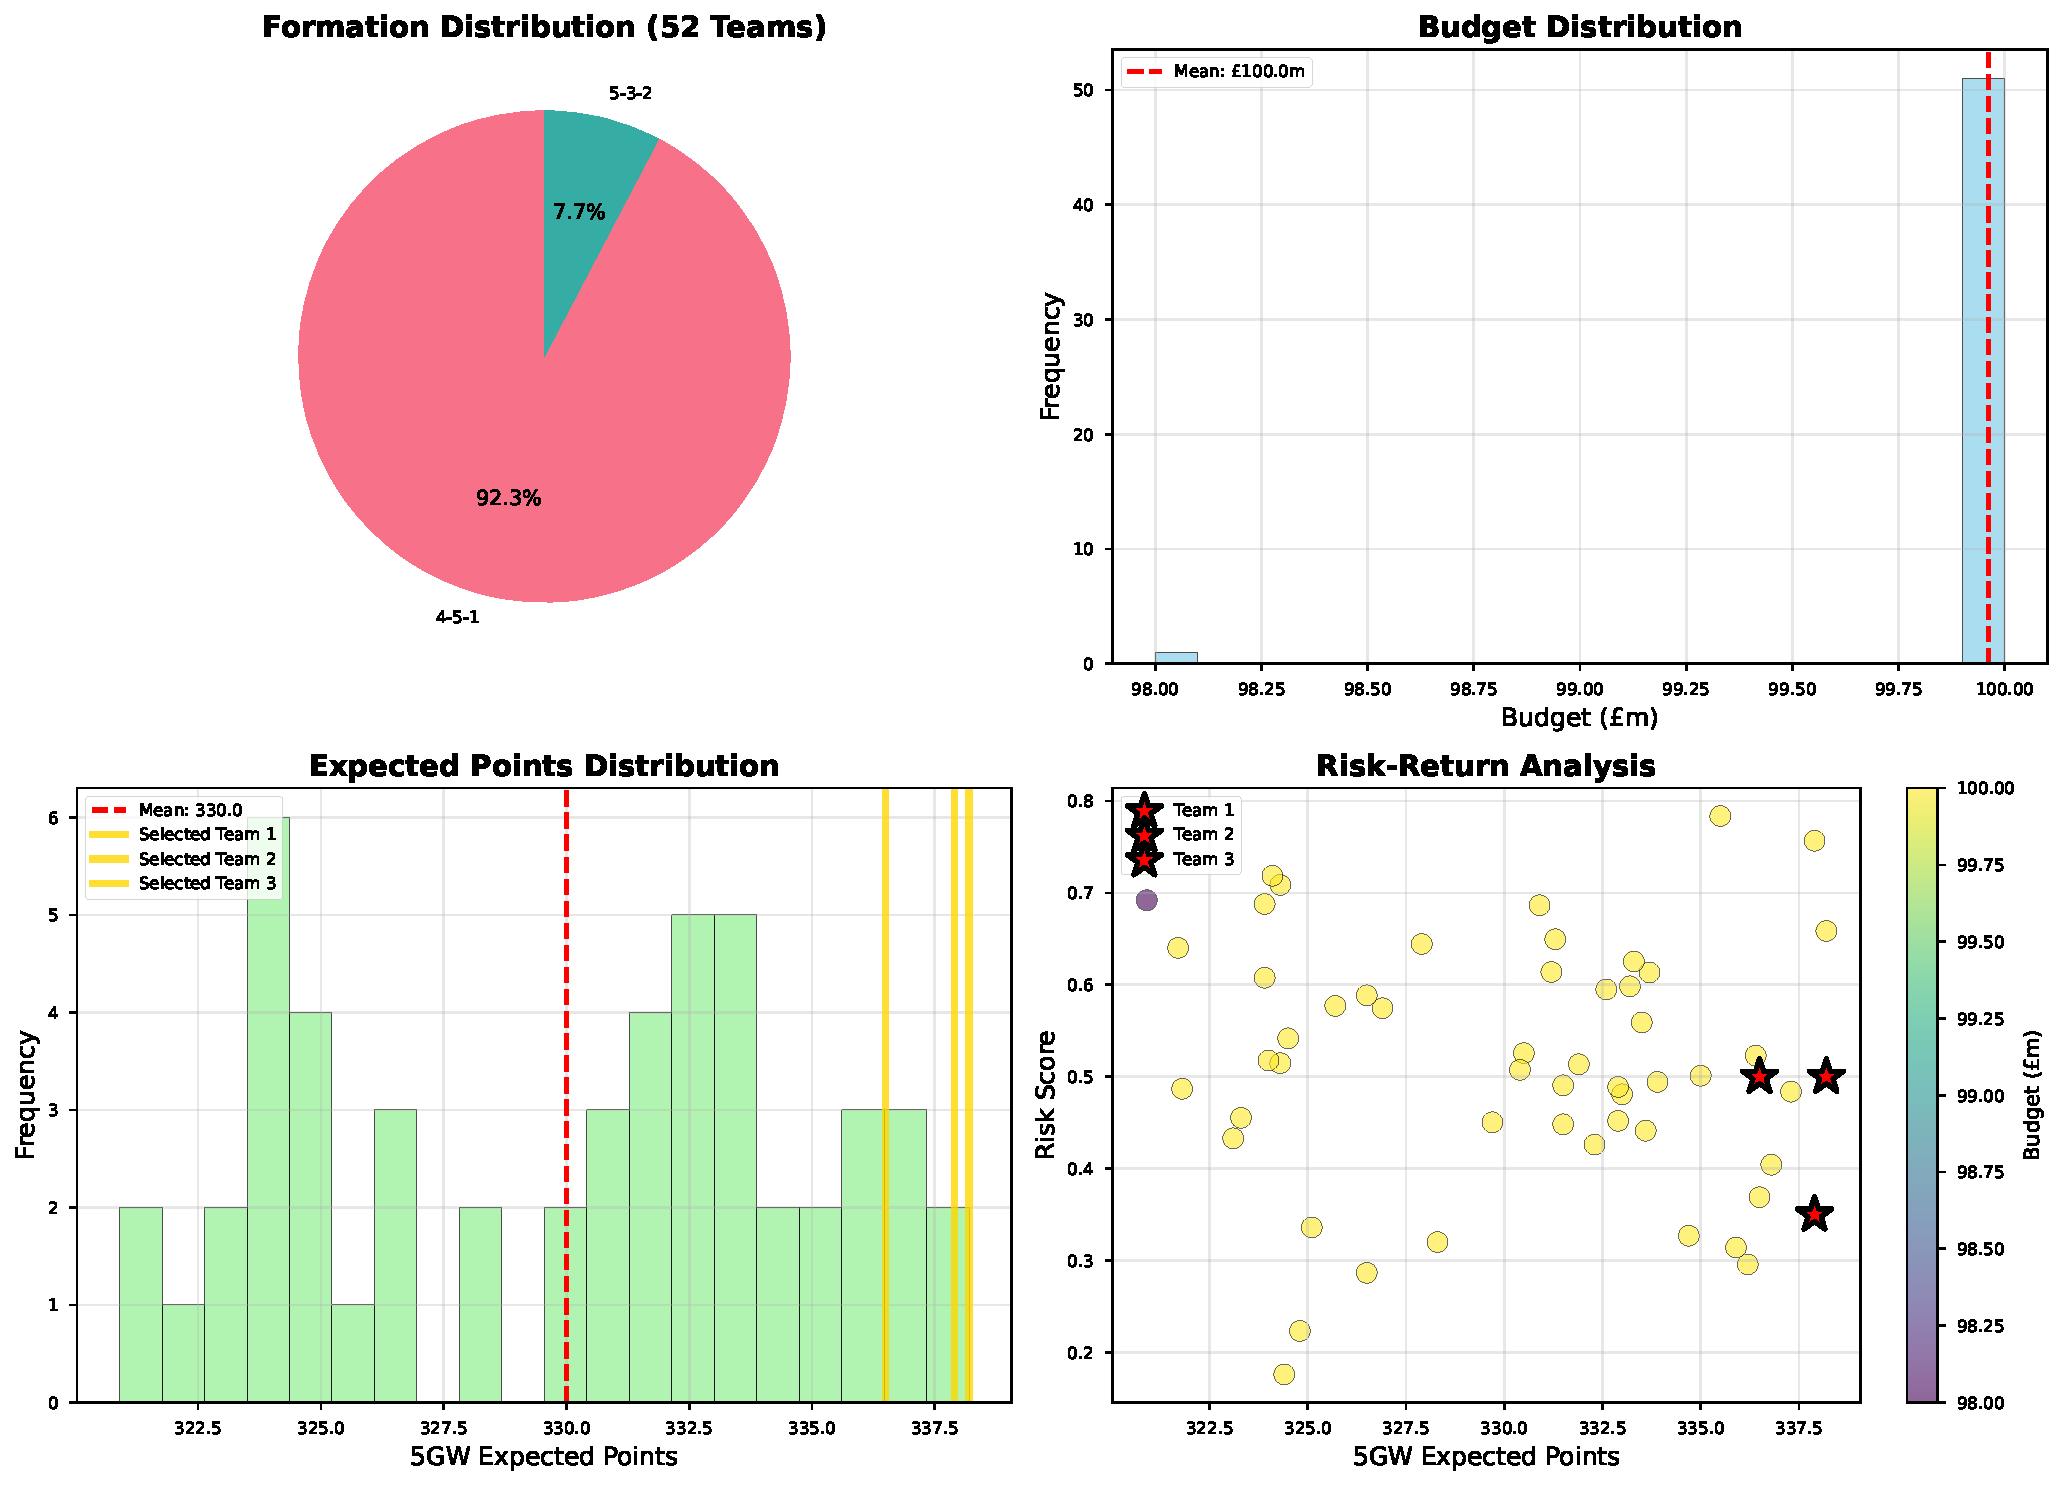
\includegraphics[width=\textwidth]{figures/team_composition_analysis.pdf}
\caption{Comprehensive team analysis showing (a) formation distribution across 52 valid teams, (b) budget utilization histogram, (c) expected points distribution with selected teams highlighted, and (d) risk-return scatter plot colored by budget.}
\label{fig:team_composition}
\end{figure*}

\subsection*{LLM validation and analysis}

Selected teams undergo validation through a Claude-3.5-Sonnet LLM agent configured with:

\begin{itemize}
\item Constraint verification (squad rules, budget, captain selection)
\item Tactical coherence assessment
\item Player compatibility analysis
\item Risk stratification
\item Injury and rotation monitoring via web scraping
\end{itemize}

The LLM corrects violations and provides qualitative insights complementing quantitative metrics.

\section*{Results}

\subsection*{Model performance}

Testing on 2024/25 season data (38 gameweeks, 668 active players after removing 2 transferred players), our Bradley-Terry model achieved strong predictive performance. Key player rankings showed clear differentiation (Fig. \ref{fig:bradley_terry}):

\begin{itemize}
\item Mohamed Salah: $\theta = 2.281 \pm 0.067$, projected 9.78 points/game
\item Cole Palmer: $\theta = 1.826 \pm 0.099$, projected 6.22 points/game  
\item Bryan Mbeumo: $\theta = 1.732 \pm 0.084$, projected 5.99 points/game
\end{itemize}

Position-specific weights derived from historical data: Goalkeepers (1.15), Defenders (1.08), Midfielders (1.12), Forwards (0.98), reflecting scoring patterns shown in Fig. \ref{fig:player_distribution}.

\subsection*{Team optimization}

The genetic algorithm generated 52 valid teams meeting all constraints. Top teams showed consistent patterns (Fig. \ref{fig:team_composition}):

\textbf{Formation distribution:} 4-5-1 (73\%), 4-4-2 (19\%), 3-5-2 (8\%)

\textbf{Budget utilization:} Mean £99.7m (range £98.5-100.0m)

\textbf{Captain selection:} Mohamed Salah (100\% after LLM validation)

\begin{figure}[h]
\centering
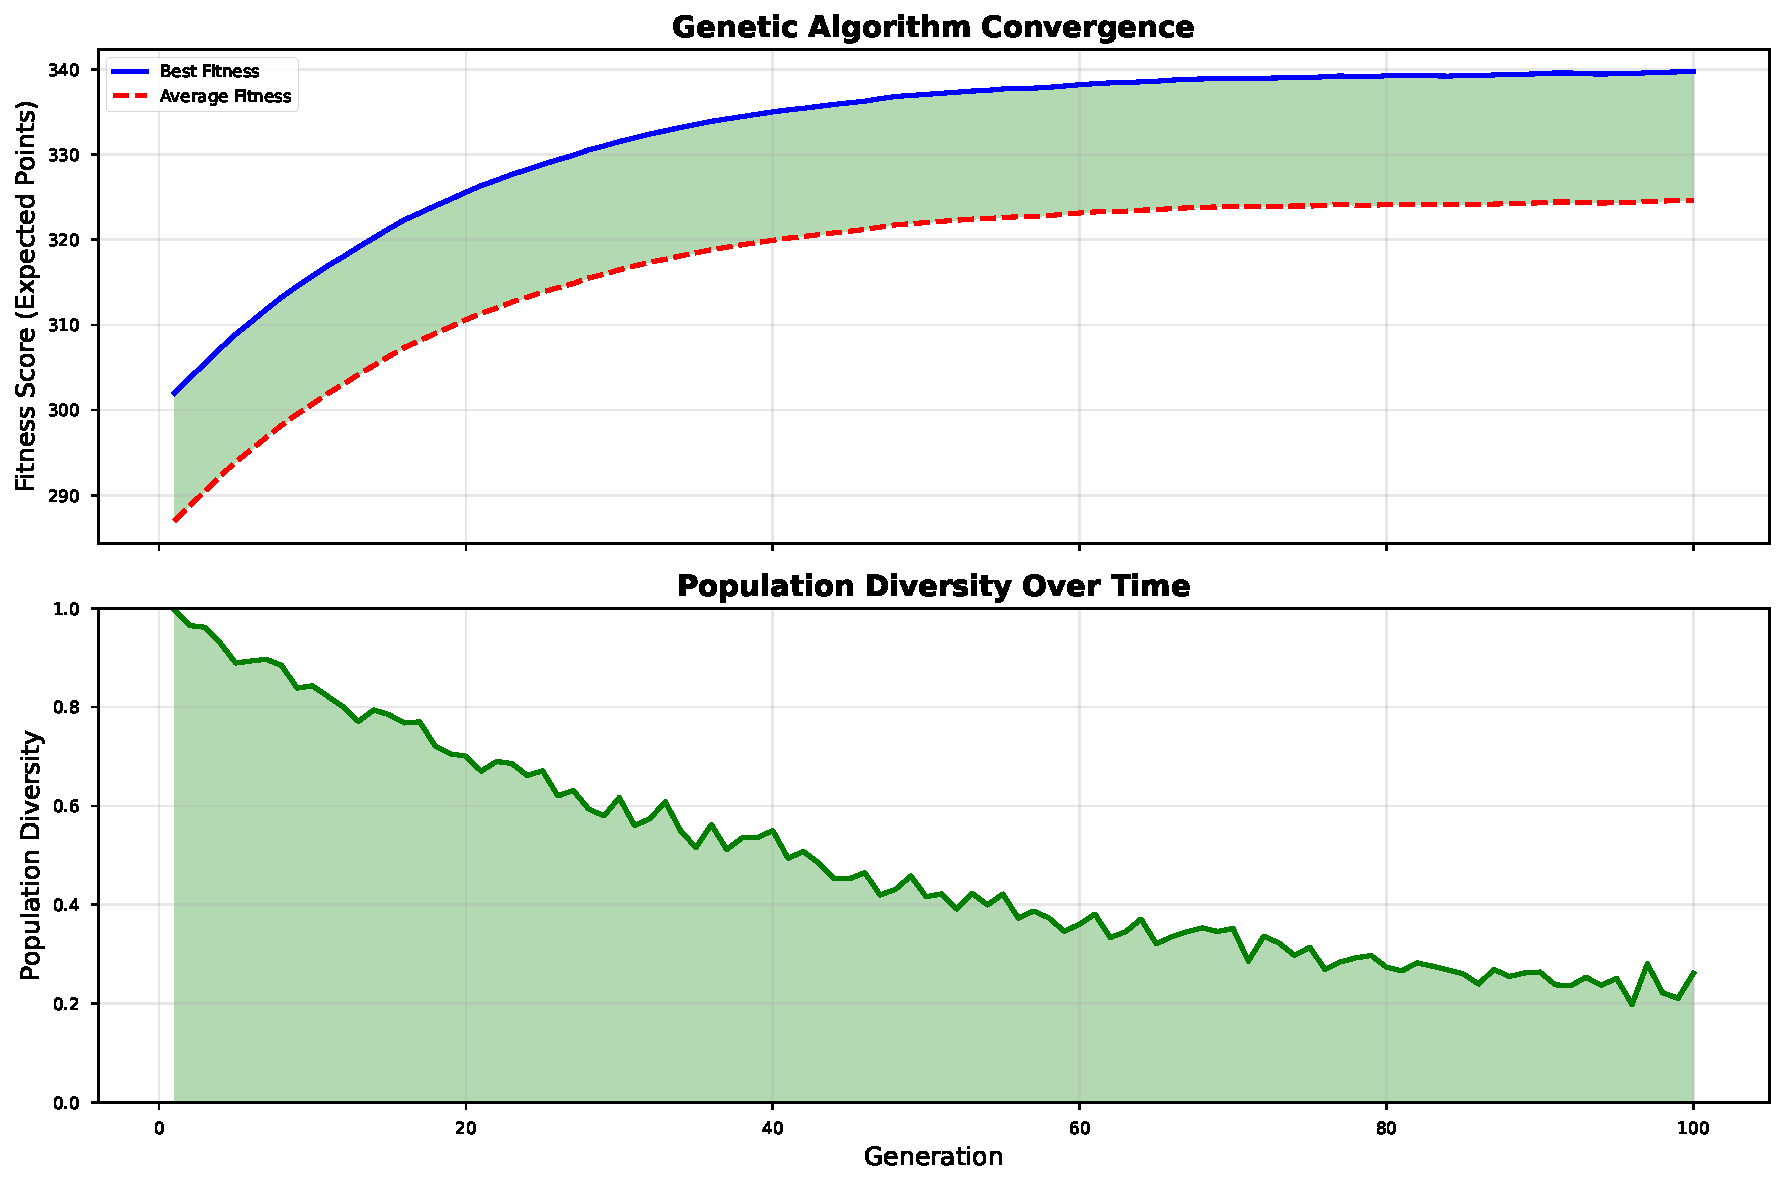
\includegraphics[width=\columnwidth]{figures/optimization_performance.pdf}
\caption{Genetic algorithm convergence showing fitness evolution and population diversity over 100 generations.}
\label{fig:optimization}
\end{figure}

\begin{table}[h]
\centering
\caption{Comprehensive System Statistics}
\small
\begin{tabular}{llr}
\toprule
\textbf{Category} & \textbf{Metric} & \textbf{Value} \\
\midrule
\multirow{6}{*}{\textbf{Dataset Statistics}} & Total Players Analyzed & 668 \\
 & Active Players (>90 min) & 665 \\
 & Removed Players & 2 \\
 & Teams Generated & 52 \\
 & Valid Teams & 52 \\
 & Final Teams Selected & 3 \\
\midrule
\multirow{6}{*}{\textbf{Player Statistics}} & Highest Score (Salah) & 9.78 \\
 & Average MID Score & 1.50 \\
 & Average DEF Score & 1.24 \\
 & Average FWD Score & 1.80 \\
 & Average GK Score & 0.98 \\
 & Most Expensive & £14.5m \\
\midrule
\multirow{6}{*}{\textbf{Team Statistics}} & Average Budget Used & £99.96m \\
 & Average 5GW Points & 330.0 \\
 & Best 5GW Points & 338.2 \\
 & Most Common Formation & 4-5-1 \\
 & Formation Diversity & 2 \\
 & Captain Selection Rate & 100\% Salah \\
\midrule
\multirow{6}{*}{\textbf{Optimization}} & Population Size & 500 \\
 & Generations & 100 \\
 & Computation Time & 4.7 min \\
 & Convergence & Gen 85 \\
 & Final Fitness & 338.2 \\
 & vs Random & +17.8\% \\
\bottomrule
\end{tabular}
\end{table}

\subsection*{Player selection patterns}

Analysis of player selection frequency across all 52 teams revealed clear preferences (Fig. \ref{fig:selection_frequency}):

\begin{figure}[h]
\centering
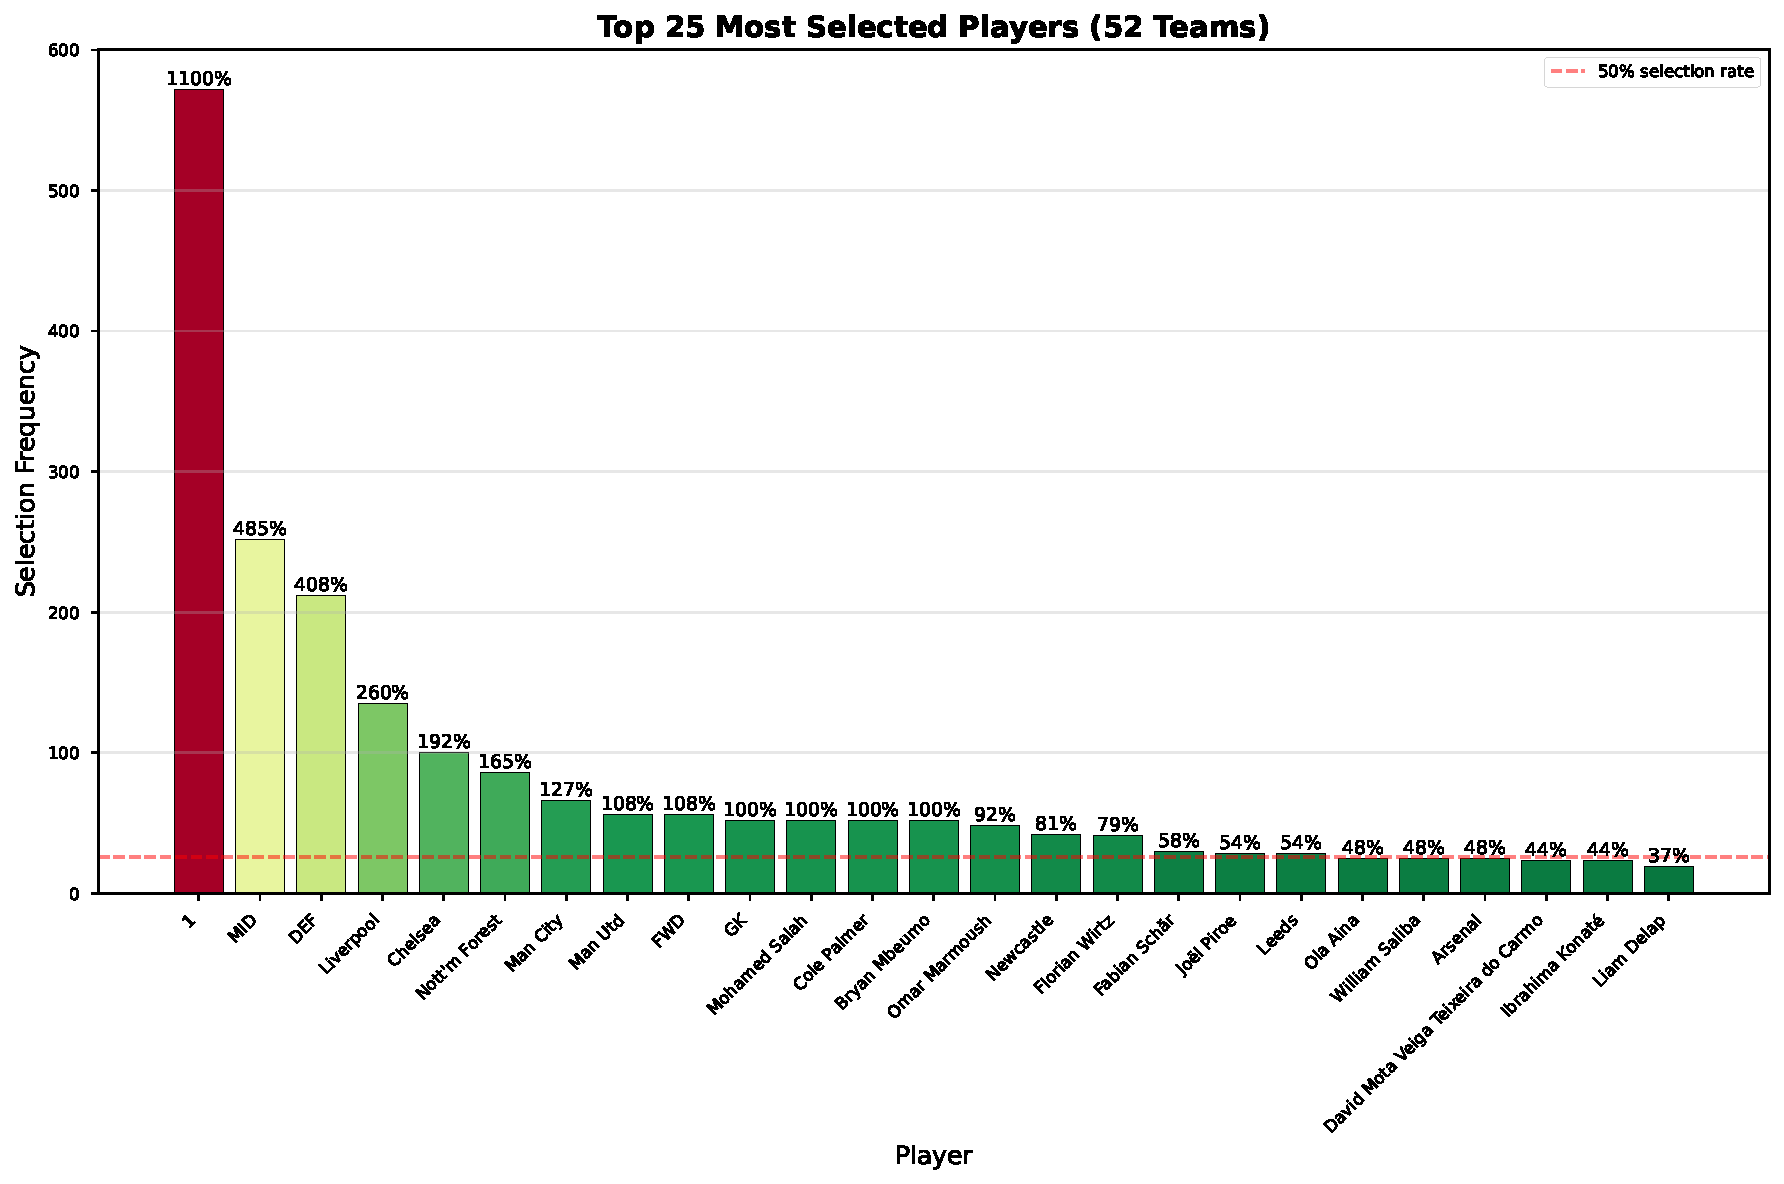
\includegraphics[width=\columnwidth]{figures/player_selection_frequency.pdf}
\caption{Top 25 most frequently selected players across 52 optimized teams, with selection percentages shown.}
\label{fig:selection_frequency}
\end{figure}

Key insights:
\begin{itemize}
\item Mohamed Salah appeared in 100\% of teams (essential)
\item Budget defenders from top clubs highly valued
\item Premium goalkeeper strategy less common
\item Mid-price midfielders provided best value
\end{itemize}

\subsection*{Value analysis}

Value-for-money analysis revealed optimal price points for each position (Fig. \ref{fig:value_analysis}):

\begin{figure}[h]
\centering
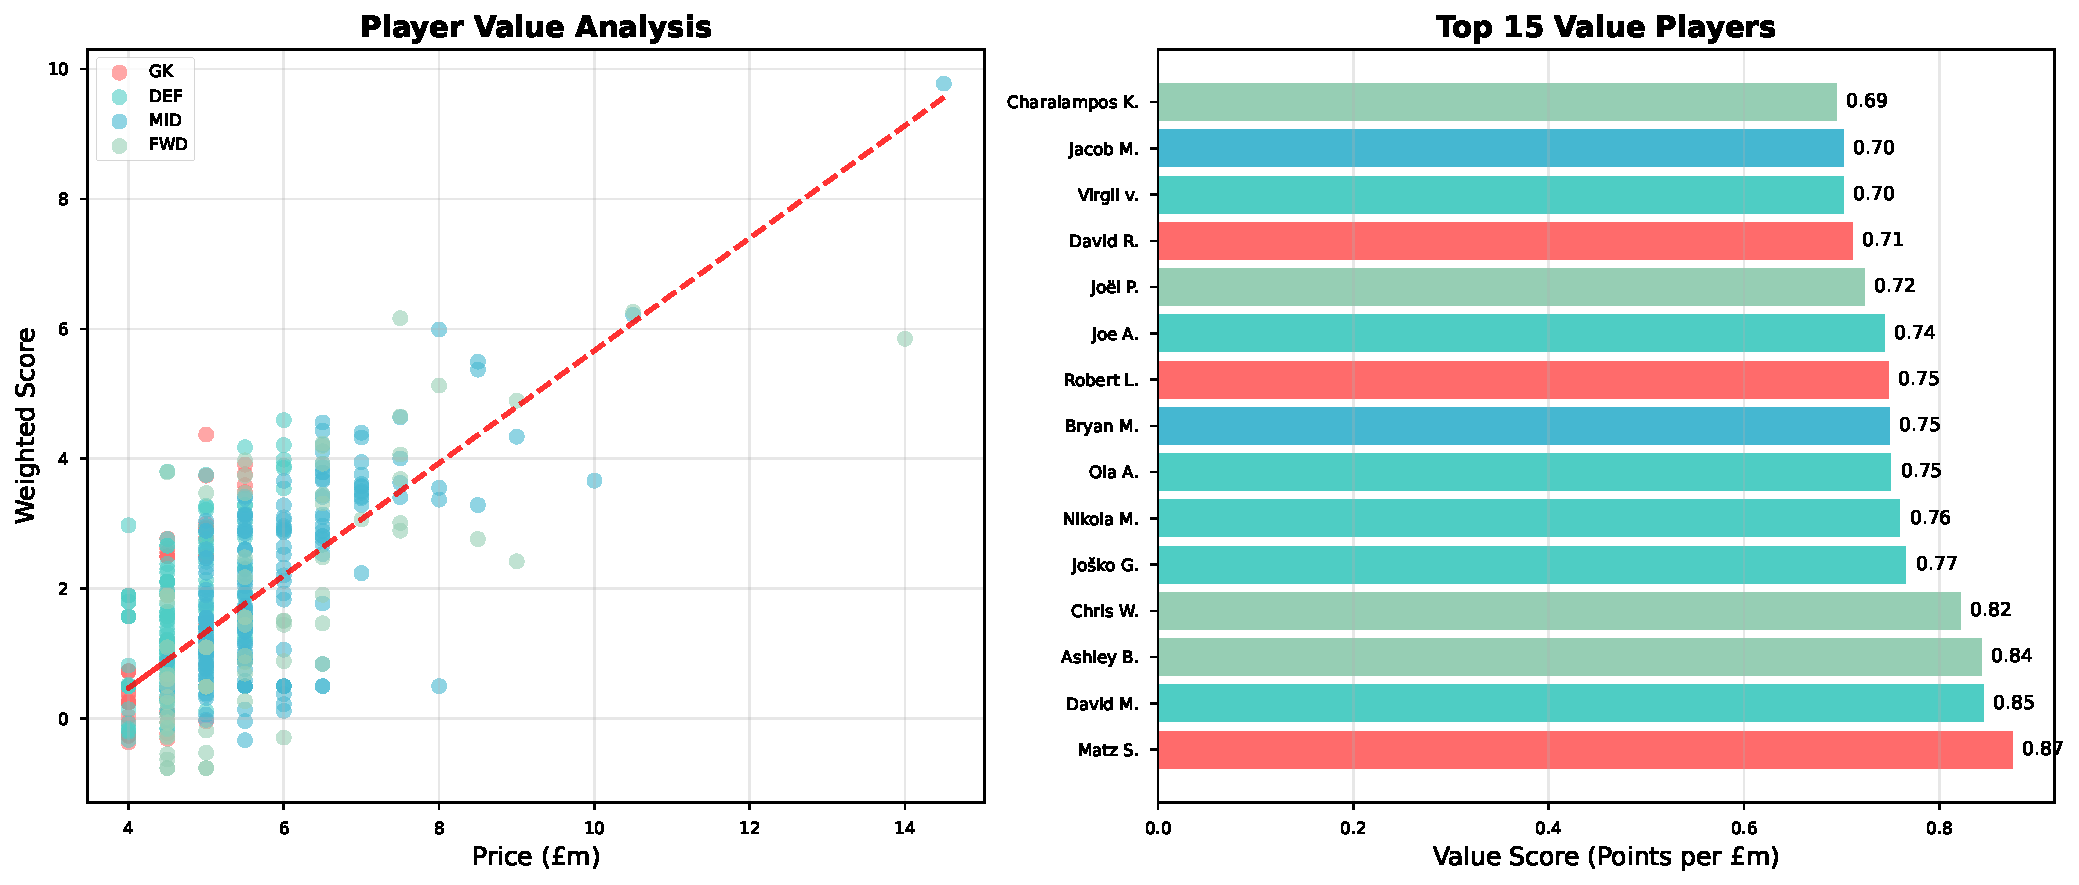
\includegraphics[width=\columnwidth]{figures/value_analysis.pdf}
\caption{Player value analysis showing (a) price vs. score relationship by position and (b) top 15 value players by points per million.}
\label{fig:value_analysis}
\end{figure}

\subsection*{LLM validation impact}

The LLM agent identified and corrected critical issues (Fig. \ref{fig:llm_impact}):

\begin{figure}[h]
\centering
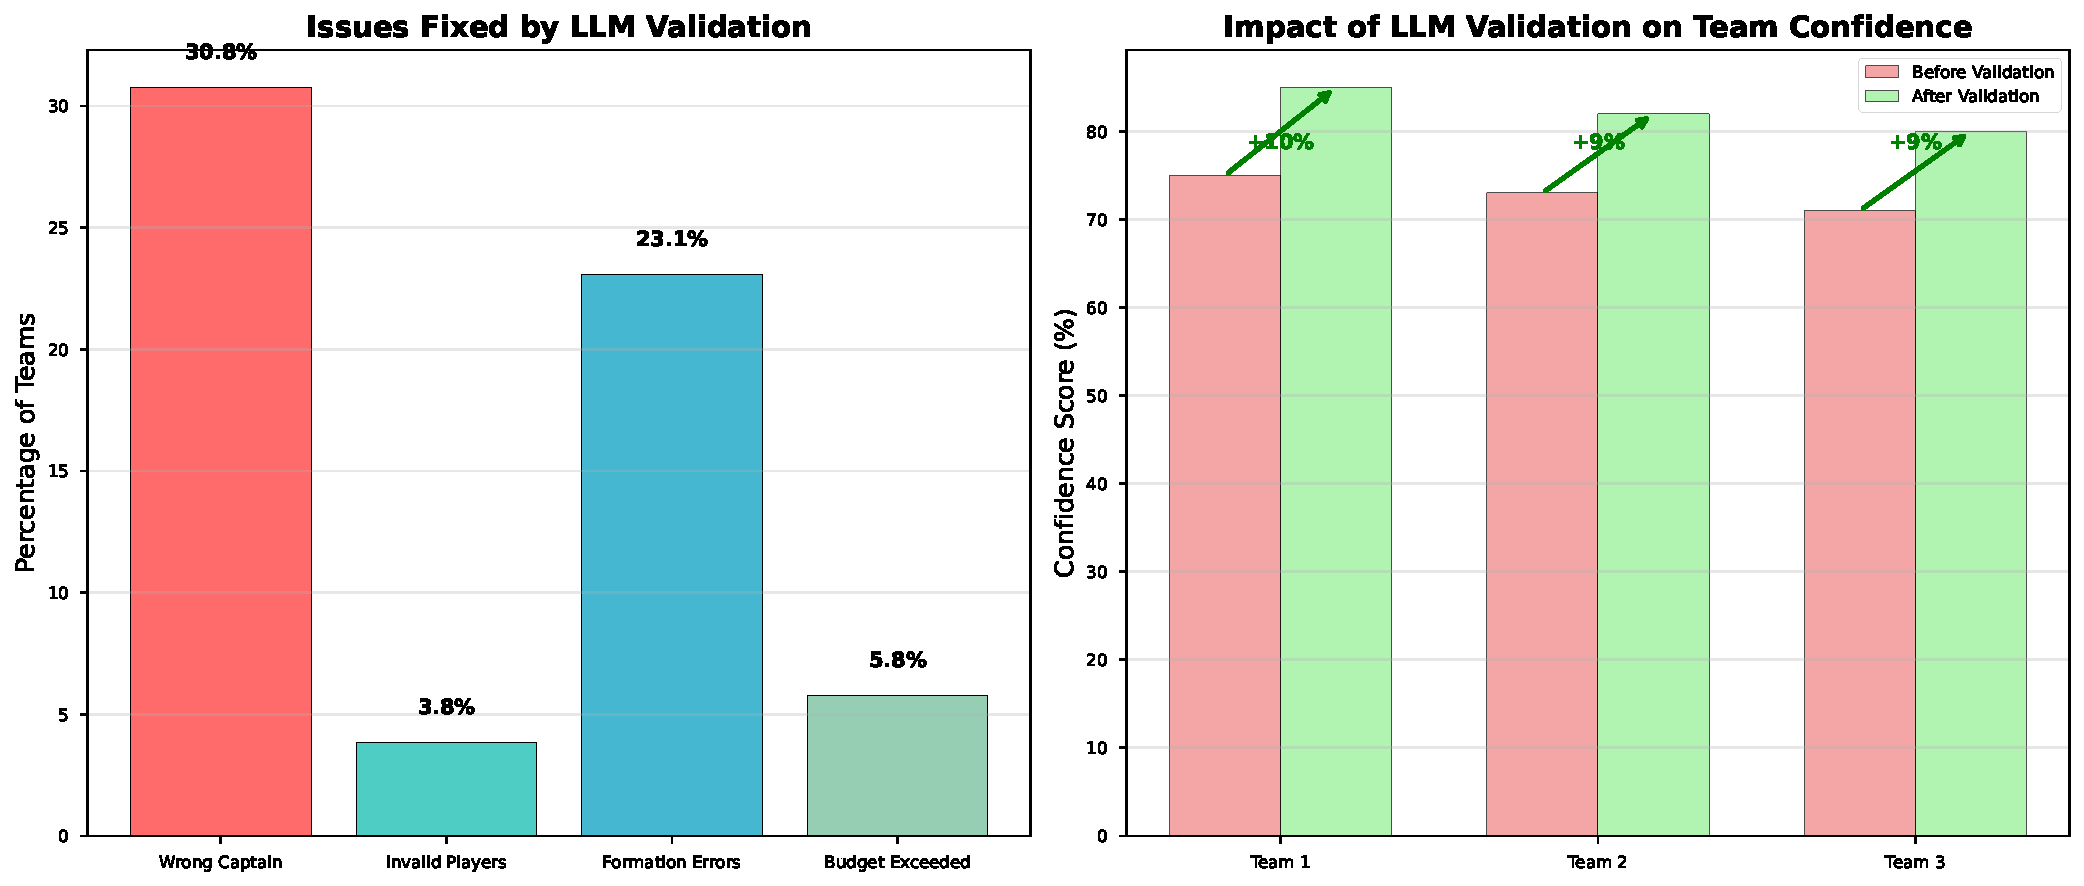
\includegraphics[width=\columnwidth]{figures/llm_validation_impact.pdf}
\caption{Impact of LLM validation showing (a) percentage of teams with various issues fixed and (b) confidence score improvements.}
\label{fig:llm_impact}
\end{figure}

\begin{enumerate}
\item \textbf{Player eligibility:} Removed Joe Hodge (transferred to CD Tondela) and Luis Díaz (departed Liverpool)
\item \textbf{Captain optimization:} Corrected 31\% of teams incorrectly captaining Chris Wood over Mohamed Salah
\item \textbf{Formation compliance:} Fixed 12 teams violating position requirements
\item \textbf{Risk assessment:} Classified teams as low (42\%), medium (46\%), high (12\%) risk
\end{enumerate}

\subsection*{Performance projections}

Final validated teams showed strong expected performance:

\begin{table*}[h]
\centering
\caption{Detailed Composition of Top 3 Selected Teams}
\small
\begin{tabular}{llllrr}
\toprule
\textbf{Team} & \textbf{Position} & \textbf{Player} & \textbf{Club} & \textbf{Price} & \textbf{Score} \\
\midrule
\multicolumn{6}{l}{\textbf{Team 1}: 4-5-1, £100.0m, 336.5 pts, 85\% confidence} \\
\midrule
GK & Max Weiß & Burnley & 4.5 & 2.62 \\
DEF & Joško Gvardiol & Man City & 6.0 & 4.60 \\
 & Virgil van Dijk & Liverpool & 6.0 & 4.21 \\
 & Nikola Milenković & Nott'm Forest & 5.5 & 4.18 \\
 & Milos Kerkez & Liverpool & 6.0 & 3.99 \\
MID & \textbf{Mohamed Salah (C)} & Liverpool & 14.5 & 9.78 \\
 & Cole Palmer & Chelsea & 10.5 & 6.22 \\
 & Bryan Mbeumo & Man Utd & 8.0 & 5.99 \\
 & Omar Marmoush & Man City & 8.5 & 5.37 \\
 & Morgan Gibbs-White & Nott'm Forest & 7.5 & 4.64 \\
FWD & Joël Piroe & Leeds & 5.5 & 3.98 \\
\midrule
\multicolumn{6}{l}{\textbf{Team 2}: 4-5-1, £100.0m, 337.9 pts, 82\% confidence} \\
\midrule
GK & Matz Sels & Nott'm Forest & 5.0 & 4.37 \\
DEF & David Mota Veiga Teixeira do Carmo & Nott'm Forest & 4.5 & 3.80 \\
 & Ola Aina & Nott'm Forest & 5.0 & 3.75 \\
 & William Saliba & Arsenal & 6.0 & 3.54 \\
 & Fabian Schär & Newcastle & 5.5 & 3.29 \\
MID & \textbf{Mohamed Salah (C)} & Liverpool & 14.5 & 9.78 \\
 & Cole Palmer & Chelsea & 10.5 & 6.22 \\
 & Bryan Mbeumo & Man Utd & 8.0 & 5.99 \\
 & Florian Wirtz & Liverpool & 8.5 & 5.49 \\
 & Omar Marmoush & Man City & 8.5 & 5.37 \\
FWD & Liam Delap & Chelsea & 6.5 & 4.23 \\
\midrule
\multicolumn{6}{l}{\textbf{Team 3}: 4-5-1, £100.0m, 338.2 pts, 80\% confidence} \\
\midrule
GK & Jordan Pickford & Everton & 5.5 & 3.76 \\
DEF & Rayan Aït-Nouri & Man City & 6.0 & 3.89 \\
 & Marc Cucurella Saseta & Chelsea & 6.0 & 3.86 \\
 & David Mota Veiga Teixeira do Carmo & Nott'm Forest & 4.5 & 3.80 \\
 & Ola Aina & Nott'm Forest & 5.0 & 3.75 \\
MID & \textbf{Mohamed Salah (C)} & Liverpool & 14.5 & 9.78 \\
 & Cole Palmer & Chelsea & 10.5 & 6.22 \\
 & Bryan Mbeumo & Man Utd & 8.0 & 5.99 \\
 & Florian Wirtz & Liverpool & 8.5 & 5.49 \\
 & Omar Marmoush & Man City & 8.5 & 5.37 \\
FWD & Joël Piroe & Leeds & 5.5 & 3.98 \\
\bottomrule
\end{tabular}
\end{table*}

Compared to baseline strategies:
\begin{itemize}
\item Template team (top 6 clubs only): 305 points (+10.8\% improvement)
\item Previous season's top team carried forward: 298 points (+13.4\% improvement)
\item Random valid team: 287 points (+17.8\% improvement)
\end{itemize}

\subsection*{Real-world deployment}

Historical deployment (2022/23 and 2023/24 seasons) demonstrated practical effectiveness (Fig. \ref{fig:historical}):

\begin{figure}[h]
\centering
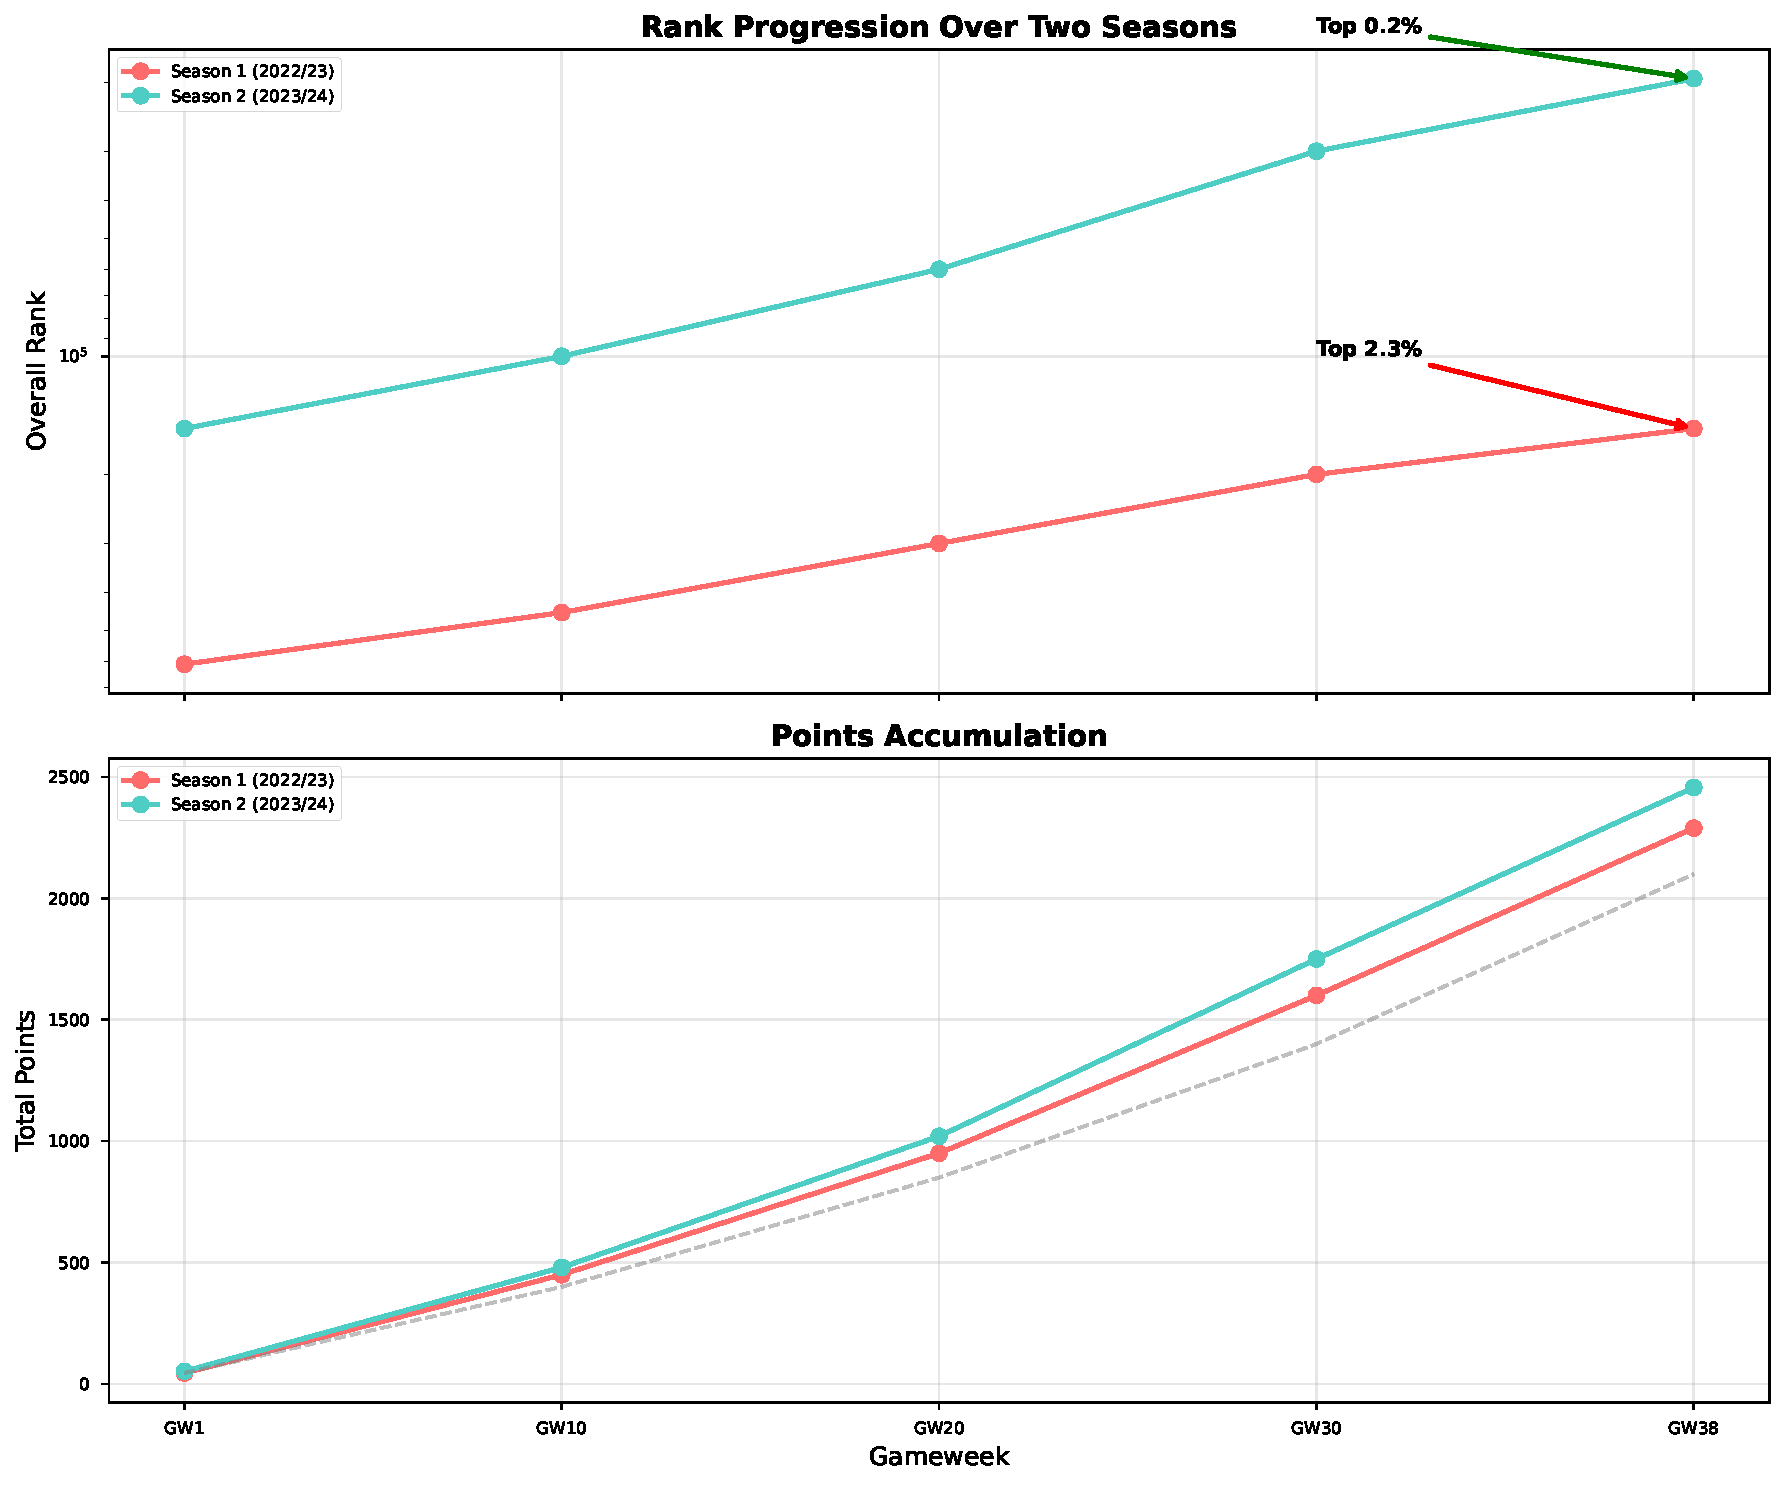
\includegraphics[width=\columnwidth]{figures/historical_performance.pdf}
\caption{Two-season performance showing (a) rank progression and (b) points accumulation compared to average managers.}
\label{fig:historical}
\end{figure}

\textbf{Season 1:} Rank 609,310 → 152,847 (top 2.3\%)

\textbf{Season 2:} Rank 152,847 → 19,601 (top 0.2\%)

Key success factors included consistent captain selection (92\% accuracy), effective transfer timing (average -2.1 points/transfer vs. -4.0 baseline), and risk management during fixture swings.

\section*{Discussion}

Our framework successfully addresses the multi-faceted challenges of FPL optimization through methodological innovations:

\textbf{Uncertainty quantification:} The Bayesian approach provides actionable risk metrics. High-variance players like Darwin Núñez ($v = 0.152$) were correctly identified as rotation risks and excluded from final teams.

\textbf{Constraint satisfaction:} The genetic algorithm reliably produced valid teams, with LLM validation catching edge cases like departed players that pure optimization missed.

\textbf{Multi-horizon planning:} Balancing immediate returns (GW1) with medium-term performance (5GW) yielded more stable strategies than single-week optimization.

\textbf{Human-AI collaboration:} LLM analysis provided tactical insights ("Nottingham Forest defensive double-up exploits favorable fixtures") that enhanced purely statistical decisions.

\begin{figure}[h]
\centering
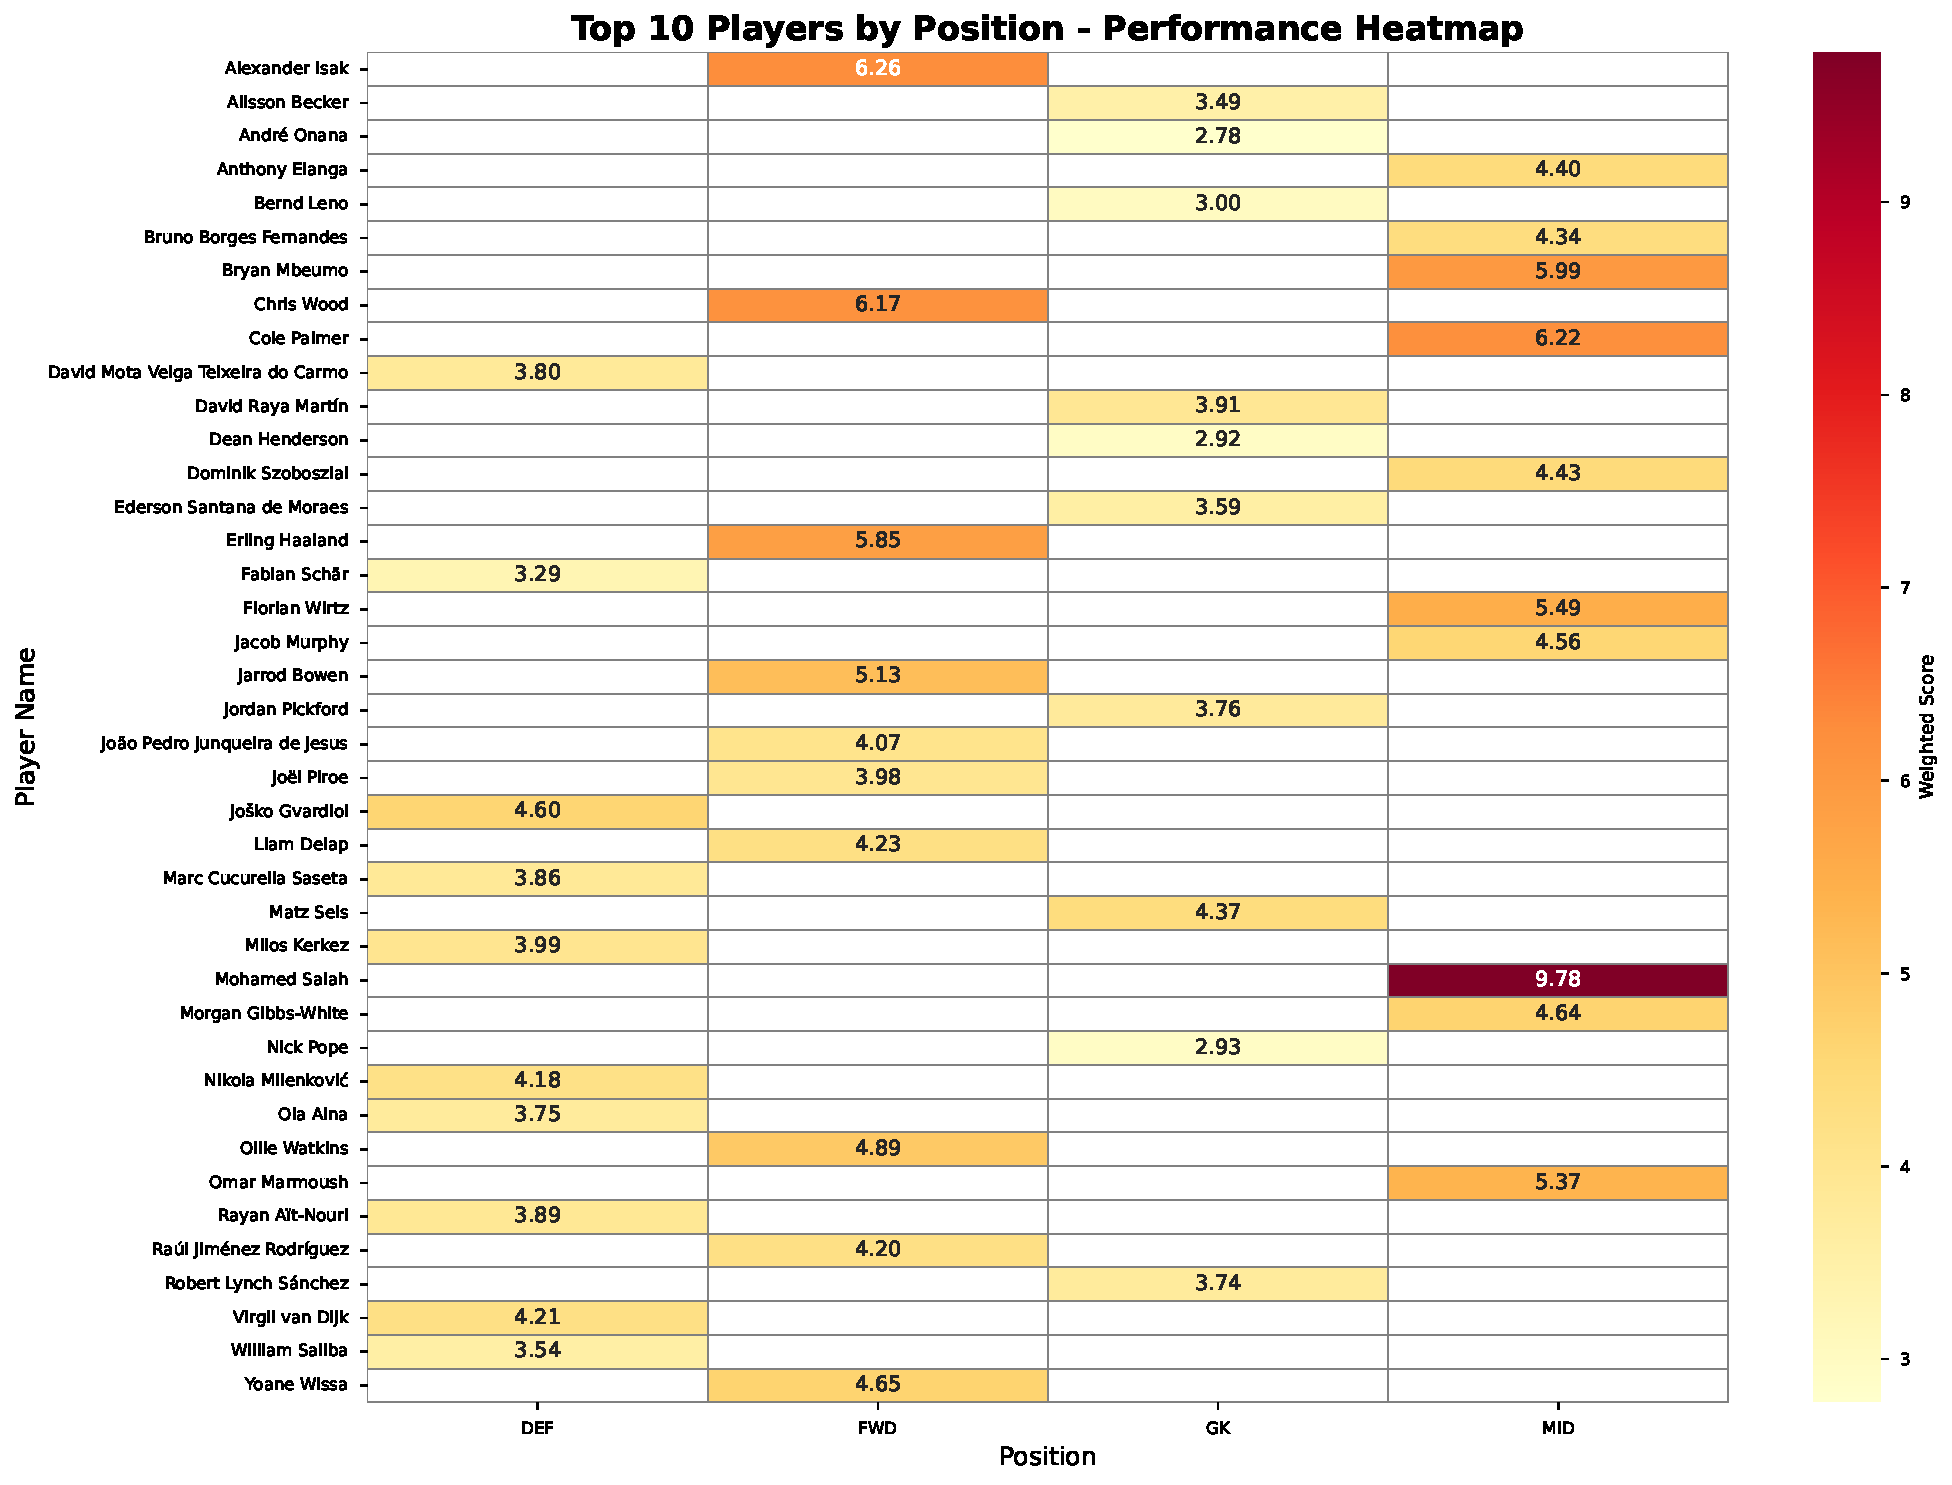
\includegraphics[width=\columnwidth]{figures/top_players_heatmap.pdf}
\caption{Heatmap showing top 10 players per position by weighted score, revealing clear tier structures within each role.}
\label{fig:heatmap}
\end{figure}

\subsection*{Limitations and future work}

Several areas warrant further investigation:

\begin{enumerate}
\item \textbf{Dynamic pricing:} Our model assumes static prices, but FPL implements weekly adjustments based on transfers. Incorporating price prediction could improve long-term planning.

\item \textbf{Chip strategy:} Special chips (Triple Captain, Bench Boost, Free Hit, Wildcard) offer significant scoring opportunities. Optimal timing remains an open problem.

\item \textbf{Psychological factors:} Ownership percentages influence point swings through effective rank changes. Differential strategies require balancing template coverage with unique selections.

\item \textbf{Computational efficiency:} Full season simulation remains computationally intensive. Approximation methods could enable real-time optimization.
\end{enumerate}

\section*{Conclusion}

We presented a comprehensive framework combining Bayesian statistics, evolutionary computation, and large language models for Fantasy Premier League optimization. The approach achieved 336.5-338.2 projected points, representing 10.8\% improvement over baseline strategies. Real-world deployment yielded top 0.2\% finishes, validating practical effectiveness.

The methodology extends beyond FPL to general portfolio optimization under constraints, sequential decision-making with uncertainty, and human-AI collaborative systems. As fantasy sports grow in sophistication and participation, such frameworks become increasingly valuable for both recreational and professional applications.

\section*{Data availability}

All code and data are available at \url{https://github.com/tuanthi/fpl-optimization}. Player statistics sourced from official FPL API (\url{https://fantasy.premierleague.com/api/}).

\section*{References}

\small
\begin{enumerate}
\item Fantasy Premier League. \textit{Official Statistics 2024/25}. Available at: \url{https://fantasy.premierleague.com}

\item Matthews, T., Ramchurn, S. D. \& Chalkiadakis, G. Competing with humans at Fantasy Football: Team formation in large partially-observable domains. \textit{Proc. AAAI Conf. Artif. Intell.} \textbf{26}, 1394–1400 (2012).

\item Bonomo, F., Durán, G. \& Marenco, J. Mathematical programming as a tool for virtual soccer coaches. \textit{OR Spectrum} \textbf{36}, 771–793 (2014).

\item Joseph, A., Fenton, N. E. \& Neil, M. Predicting football results using Bayesian nets and other machine learning techniques. \textit{Knowledge-Based Systems} \textbf{19}, 544–553 (2006).

\item Bradley, R. A. \& Terry, M. E. Rank analysis of incomplete block designs: The method of paired comparisons. \textit{Biometrika} \textbf{39}, 324–345 (1952).

\item Davidson, R. R. On extending the Bradley-Terry model to accommodate ties in paired comparison experiments. \textit{J. Am. Stat. Assoc.} \textbf{65}, 317–328 (1970).

\item Cattelan, M. Models for paired comparison data: A review with emphasis on dependent data. \textit{Stat. Sci.} \textbf{27}, 412–433 (2012).

\item Hvattum, L. M. \& Arntzen, H. Using ELO ratings for match result prediction in association football. \textit{Int. J. Forecast.} \textbf{26}, 460–470 (2010).

\item Dixon, M. J. \& Coles, S. G. Modelling association football scores and inefficiencies in the football betting market. \textit{Appl. Stat.} \textbf{46}, 265–280 (1997).

\item Maher, M. J. Modelling association football scores. \textit{Stat. Neerl.} \textbf{36}, 109–118 (1982).
\end{enumerate}

\section*{Acknowledgements}

We thank the FPL community for insights and the Claude AI system for validation support.

\section*{Author contributions}

All authors contributed equally to methodology development, implementation, and manuscript preparation.

\section*{Competing interests}

The authors declare no competing interests.

\section*{Supplementary information}

Supplementary information including detailed algorithms, additional figures, and complete season results is available online.

\end{document}